\chapter{Complementary Results}
\label{Complementary_Results}

\section{Changing the vortices' topological charge $\ell$}

\begin{figure}[htbp]
    \centering
    \begin{subfigure}[b]{0.45\textwidth}
        \centering
        \includegraphics[width=\textwidth]{images/Appendices/Additional_Results/Topological_Charge/type=0_r=0_zi=0_zf=1000.eps}
        \caption{Regular vortex.}
    \end{subfigure}
    \hfill
    \begin{subfigure}[b]{0.45\textwidth}
        \centering
        \includegraphics[width=\textwidth]{images/Appendices/Additional_Results/Topological_Charge/type=1_r=0_zi=0_zf=1000.eps}
        \caption{Perfect vortex.}
    \end{subfigure}
    \caption{Unobstructed vortices of topological charge $\ell = 6$.}
    \label{fig:L=6_r=0}
\end{figure}

\begin{figure}[htbp]
    \centering
    \begin{subfigure}[b]{0.45\textwidth}
        \centering
        \includegraphics[width=\textwidth]{images/Appendices/Additional_Results/Topological_Charge/type=0_r=30_zi=0_zf=1000.eps}
        \caption{Regular vortex.}
    \end{subfigure}
    \hfill
    \begin{subfigure}[b]{0.45\textwidth}
        \centering
        \includegraphics[width=\textwidth]{images/Appendices/Additional_Results/Topological_Charge/type=1_r=30_zi=0_zf=1000.eps}
        \caption{Perfect vortex.}
    \end{subfigure}
    \caption{Vortices of topological charge $\ell = 6$ and obstruction radius $r = 30$ [px].}
    \label{fig:L=6_r=30}
\end{figure}

\begin{figure}[htbp]
    \centering
    \begin{subfigure}[b]{0.45\textwidth}
        \centering
        \includegraphics[width=\textwidth]{images/Appendices/Additional_Results/Topological_Charge/type=0_r=50_zi=0_zf=1000.eps}
        \caption{Regular vortex.}
    \end{subfigure}
    \hfill
    \begin{subfigure}[b]{0.45\textwidth}
        \centering
        \includegraphics[width=\textwidth]{images/Appendices/Additional_Results/Topological_Charge/type=1_r=50_zi=0_zf=1000.eps}
        \caption{Perfect vortex.}
    \end{subfigure}
    \caption{Vortices of topological charge $\ell = 6$ and obstruction radius $r = 50$ [px].}
    \label{fig:L=6_r=50}
\end{figure}

\begin{figure}[htbp]
    \centering
    \begin{subfigure}[b]{0.45\textwidth}
        \centering
        \includegraphics[width=\textwidth]{images/Appendices/Additional_Results/Topological_Charge/type=0_r=70_zi=0_zf=1000.eps}
        \caption{Regular vortex.}
    \end{subfigure}
    \hfill
    \begin{subfigure}[b]{0.45\textwidth}
        \centering
        \includegraphics[width=\textwidth]{images/Appendices/Additional_Results/Topological_Charge/type=1_r=70_zi=0_zf=1000.eps}
        \caption{Perfect vortex.}
    \end{subfigure}
    \caption{Vortices of topological charge $\ell = 6$ and obstruction radius $r = 70$ [px].}
    \label{fig:L=6_r=70}
\end{figure}


\newpage
\section{Changing perfect vortices' fundamental parameters}
\subsection{Changing regular vortices' Gaussian size}

\begin{figure}[htbp]
    \centering
    \includegraphics[width=12cm]{images/Appendices/Additional_Results/Sigma_150/type=0_r=0_zi=0_zf=1000.eps}
    \caption{Unobstructed regular vortex with Gaussian's $\sigma = 150$.}
    \label{fig:reg_s=150_r=0}
\end{figure}

\begin{figure}[htbp]
    \centering
    \includegraphics[width=12cm]{images/Appendices/Additional_Results/Sigma_150/type=0_r=30_zi=0_zf=1000.eps}
    \caption{Regular vortex with Gaussian's $\sigma = 150$ and obstruction radius $r=30$ [px].}
    \label{fig:reg_s=150_r=30}
\end{figure}

\begin{figure}[htbp]
    \centering
    \includegraphics[width=12cm]{images/Appendices/Additional_Results/Sigma_150/type=0_r=50_zi=0_zf=1000.eps}
    \caption{Regular vortex with Gaussian's $\sigma = 150$ and obstruction radius $r=50$ [px].}
    \label{fig:reg_s=150_r=50}
\end{figure}

\begin{figure}[htbp]
    \centering
    \includegraphics[width=12cm]{images/Appendices/Additional_Results/Sigma_150/type=0_r=70_zi=0_zf=1000.eps}
    \caption{Regular vortex with Gaussian's $\sigma = 150$ and obstruction radius $r=70$ [px].}
    \label{fig:reg_s=150_r=70}
\end{figure}

\begin{figure}[htbp]
    \centering
    \includegraphics[width=12cm]{images/Appendices/Additional_Results/Sigma_150/type=0_r=100_zi=0_zf=1000.eps}
    \caption{Regular vortex with Gaussian's $\sigma = 150$ and obstruction radius $r=100$ [px].}
    \label{fig:reg_s=150_r=100}
\end{figure}

\newpage
\subsection{Changing perfect vortices' aperture and number of rings}
The following set of figures show perfect vortices made with an aperture of $Rpx = 500$ [px] and number of rings $N = 60$. The first figure is propagated through $z = 1000$ [mm] and it clearly shows that altering the fundamental parameters distorts the vortex in a negative ways.



To counter arrest this effect, it is necessary to decrease the propagation distance to $z = 600$ [mm]. The following set of figures shows the evolution of the perfect vortices with growing obstruction sizes, considering the parameters described at the beginning of this subsection and the new propagation distance.



\section{Staged propagation results}